\section{The other lineage: search at play time, value networks at the horizon}\label{sec:search}

\mkey{why search is hard here}Deep CFR \emph{amortizes}: all solving happens in training, and play is a forward pass. The rival lineage --- the one behind DeepStack, Libratus, and today's GTO Wizard AI --- \emph{searches}: solve the situation you are actually in, at play time, the way chess engines do. In poker that idea breaks twice before it works. First, you never know which state you are in, so search must reason over \emph{ranges} (Section~\ref{sec:solving}'s probability cloud) rather than positions. Second, and less obviously:

\begin{intuition}{why you cannot just solve the river when you get there}
How an opponent plays a river depends on rivers that never happened --- if your new river strategy stops paying off their bluffs, then \emph{arriving} at this river with bluffs was a mistake for them, and a rational opponent's whole earlier game shifts. Solve the subgame ``optimally'' in isolation and you can make your \emph{overall} strategy more exploitable. The 2014 fix (Burch et al.~\cite{burch2014}) is a buyout clause: re-solve the subgame under a constraint that at its entrance, every opponent hand may either play on into your new strategy or take a ``buyout'' equal to what that hand was worth under your old strategy. If no hand prefers deviating, your new strategy concedes nothing it had not already conceded --- \emph{safe re-solving}, the gadget every sound search method builds on.
\end{intuition}

With safety available, the lineage is a sequence of ways to stop searching early (Figure~\ref{fig:lineage} maps it):

\begin{itemize}
\item \textbf{DeepStack} (2017~\cite{deepstack}): re-solve a small lookahead at \emph{every} decision (``continual resolving''), carrying only your range and the opponent's buyout values forward; where the lookahead ends, a \keyterm{counterfactual value network}\mdef{counterfactual value net}{maps (pot, board, both ranges) $\to$ per-hand values --- a learned evaluation function over ranges} estimates the rest. First expert-level HUNL win; the net's input is both players' full range vectors.
\item \textbf{Libratus} (2017~\cite{libratus}): superhuman with \emph{zero} neural networks --- an abstraction blueprint (MCCFR), plus \emph{nested} safe re-solving that spawns a finer subgame solve every time the opponent does anything (including bet sizes outside the blueprint's menu, retiring action translation), plus overnight self-repair of the blueprint where opponents probed. Proof that search, not deep learning, was the load-bearing superhuman ingredient.
\item \textbf{Depth-limited solving} (2018~\cite{brown2018dls}): the cheap trick --- at the depth limit, instead of a value net, let the opponent choose among a handful of precomputed \emph{continuation strategies} (an adversarial ``several ways the rest could play''). Modicum beat top prior bots on a 4-core laptop; Pluribus (2019~\cite{pluribus}) rode the same recipe to 6-max on commodity hardware.
\item \textbf{ReBeL} (2020~\cite{rebel}): the clean theory --- recast poker as a perfect-information game over \keyterm{public belief states}\mdef{public belief state}{public observations + both players' hand distributions: a state everyone CAN see} and run AlphaZero's loop (self-play + search + value/policy nets) on that transformed game, with a Nash convergence proof. \textbf{Student of Games} (2023~\cite{sog}) generalized the recipe to chess, Go, HUNL, and Scotland Yard with one algorithm.
\item \textbf{GTO Wizard AI} (commercial, ex-Ruse~\cite{gtowizardai}): the deployed endpoint --- solves street-by-street in real time with self-play-trained value networks standing in for future streets; self-reported: arbitrary stacks and bet sizes, $\sim$3s per street, rivers solved exactly, +19.4bb/100 over Slumbot. No paper, so treat all numbers as vendor claims; the \emph{architecture pattern} is the public part.
\end{itemize}

\begin{fullbleed}
\begin{figure}[t]
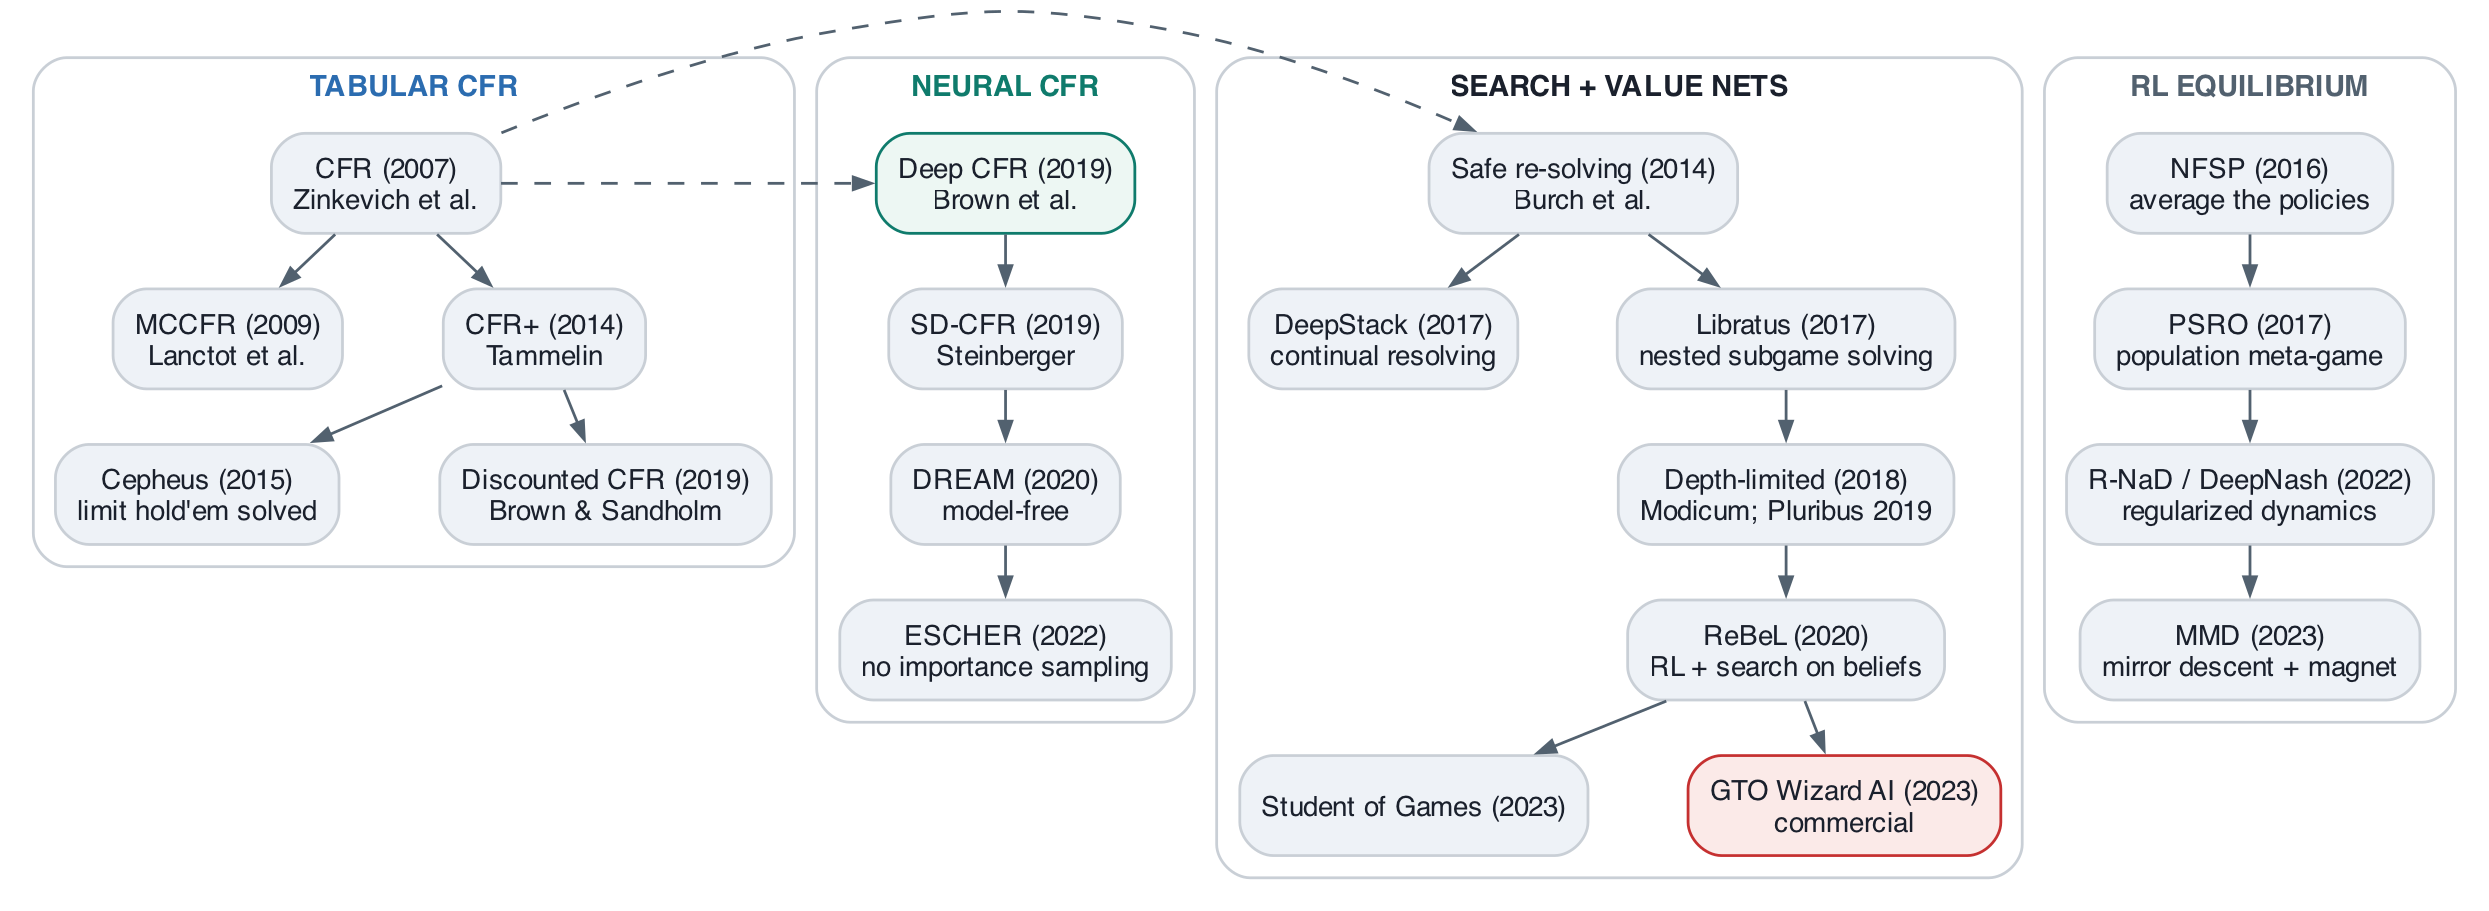
\includegraphics[width=6.45in]{figures/lineage.png}
\caption{The four method families and their landmark systems; dashed arrows mark CFR's ideas feeding the other lineages.}
\label{fig:lineage}
\end{figure}
\end{fullbleed}

\subsection*{Amortized vs.\ search: the actual tradeoff, and the Drawmaha verdict}

\begin{center}
\footnotesize
\begin{tabular}{@{}lll@{}}
\toprule
 & Amortized policy (Deep CFR) & Search + values (DeepStack/ReBeL) \\
\midrule
Per-query cost & one forward pass, ms & a subgame solve, seconds \\
Errors at play & baked in at training & partially corrected by search \\
Off-menu spots & needs action translation & re-solves them natively \\
Engineering & one training loop & belief tracking + gadgets + nested solves \\
Range input & never materialized & \textbf{2{,}598{,}960-dim vectors} \\
\bottomrule
\end{tabular}
\end{center}

\mkey{the 2.6M-dim wall}The last row is the Drawmaha-specific wall: every neural system in this lineage feeds \emph{range vectors} into its networks --- 1{,}326 dimensions in hold'em, \textbf{2{,}598{,}960} in Drawmaha (5.2M for both players). Nothing ports without aggressive hand bucketing or a factorized belief representation first, and that is the single biggest open design problem for any future Drawmaha search layer. Working in search's favor: the public draw count slots perfectly into public-belief-state bookkeeping, pot-limit bounds the bet-size branching, and the post-draw game is comparatively small. \mnote{Ranked future upgrades, cheapest first: (1) depth-limited resolve at the draw boundary using the Deep CFR net $\pm$ perturbations as continuation strategies; (2) a post-draw value net, DeepStack-style; (3) full belief-state search.}\hlight{The project's verdict, echoing the commercial history: amortized Deep CFR first --- search is the accuracy upgrade you buy later, not the foundation you start on.} One honest caveat travels with any future resolve layer: updating the opponent's range \emph{through} a hidden discard (they drew two --- which two?) is a belief-update computation no paper writes down for poker draws; Section~\ref{sec:checklist} carries it as an open problem.
